\documentclass{article}
\usepackage{graphicx}
\usepackage{wrapfig}
\usepackage{subcaption}
\usepackage{geometry}
\geometry{legalpaper, margin=1in}
\usepackage{amsmath} % or simply amstext
\newcommand{\angstrom}{\textup{\AA}}
\title{Predicting Transport in Lyotropic Liquid Crystal Membranes with Molecular Dynamics Simulations -- Outline}
\author{Benjamin J. Coscia \and Douglas L. Gin \and Richard D. Noble \and Joe Yelk \and Matthew Glaser \and Xunda Feng \and Michael R. Shirts} 
\begin{document}
  \bibliographystyle{ieeetr}
  \graphicspath{{./figures/}}
  \maketitle
  \section*{Introduction}
  
  Nanostructured membrane materials have become increasingly popular for 
  aqueous separations applications such as desalination and biorefinement
  because they offer the ability to control membrane architecture at the
  atomic scale allowing the design of solute-specific separation membranes. \cite{humplik_nanostructured_2011}
  \begin{itemize}
    \item Most membrane-based aqueous separations of small molecules can 
    be achieved using reverse osmosis (RO) or nanofiltration (NF) \cite{van_der_bruggen_review_2003}
  \end{itemize}
  
  While RO and NF have seen many advances in the past few decades, they 
  are far from perfect separation technologies.
  \begin{itemize}
    \textit{RO membranes}
    \item \textbf{Inconsistent performance} : Current state-of-the-art RO membranes are unstructured with
    tortuous and polydisperse diffusion pathways which leads to 
    inconsistent performance \cite{song_nano_2011}
    \item \textbf{High energy requirements} : Necessarily high feed pressures 
    drive up energy requirements which strains developing regions and
    contributes strongly to CO\textsubscript{2} emissions. \cite{mcginnis_global_2008}
    \item \textbf{Separation based on differences in solubility and diffusivity:
    Moreover, designing RO membranes to achieve targeted separations of 
    specific solutes is nearly impossible because various solutes dissolve
    into and diffuse through the polymer matrix at different rates. \cite{wijmans_solution-diffusion_1995}
    \item At best, one can exploit these differences to create a functional
    selective barrier.
    \textit{NF membranes}
    \item NF was introduced as an intermediate between RO and ultrafiltration,
    having the ability to separate organic matter and salts on the order of 
    one nanometer in size.
    \item Larger and well-defined pores drive down energy requirements while
    still affording separation of solutes as small as ions to some degree \cite{van_der_bruggen_review_2003}
    \item NF is often used as a precursor to reverse osmosis
    \item Unfortunately, NF membranes, like RO, are produced with a pore size 
    distribution which limits their ability to perform precise separations \cite{bowen_modelling_2002}
  \end{itemize}
  
  Nanostructured membranes can bypass many of the performance issues which
  plague traditional NF and RO membranes.
  \begin{itemize}
    \item \textbf{Tune size and functionality of building blocks} to control pore
    size and shape: One can accomplish targeted separations with high 
    selectivity by tuning shape, size and functionality of the molecular
    building blocks which form these materials. % BJC: "these materials" --> "nanostructured membranes", or is that redundant?
    \item As a result, solute rejecting pores can have their sizes tuned
    uniformly, resulting in \textbf{strict size cut-offs}.
    \item Entirely \textbf{different mechanisms} may govern transport in a given
    nanostructured material which can inspire novel separation techniques.
  \end{itemize}
  
  Development of nanostructured materials has been limited by the ability
  to synthesize and scale various fundamentally sound technologies.
  \begin{itemize}
    \item \textbf{Graphene sheets} are atomically thick which results in excellent
    permeability but defects during manufacturing severely impact 
    selectivity. \cite{cohen-tanugi_multilayer_2016}
    \item Molecular dynamics simulations of \textbf{carbon nanotubes} show
    promise \cite{humplik_nanostructured_2011} but synthetic techniques are 
    unable to achieve scalable alignment and pore monodispersity.\cite{hata_water-assisted_2004,maruyama_growth_2005}
    \item \textbf{Zeolites} have sub-nm pores with a narrow pore size 
    distribution and MD simulations exhibit complete rejection of solvated ions, \cite{murad_molecular_1998}
    however, experimental rejection was low and attributed to interstitial
    defects formed during membrane synthesis \cite{li_desalination_2004}
    \item There is a need for a scalable nanostructured membrane
  \end{itemize}
  
  Self assembling lyotropic liquid crystals (LLCs) are a suitable candidate for
  aqueous separation applications. 
  \begin{itemize}
    \item LLCs share the characteristic ability of nanostructured membrane
    materials to create \textbf{highly ordered structures} with the added benefits
    of \textbf{low cost} and synthetic techniques feasible for 
    \textbf{large scale production} \cite{feng_scalable_2014}
    \item Neat liquid crystal monomer forms the thermotropic, Col\textsubscript{h}
    phase. The presence of small amounts of water results in the H\textsubscript{II} 
    phase.
    \item In both cases, monomers assemble into mesophases made of hexagonally
    packed, uniform size, cylinders with hydrophilic groups oriented inward
    towards the pore center and hydrophobic groups facing outward.
    \item H\textsubscript{II} and Col\textsubscript{h} phase systems created by
    the monomer named Na-GA3C11 has been extensively studied experimentally \cite{smith_ordered_1997, %BJC: IUPAC chemical name here?
    zhou_supported_2005,resel_h2-phase_2000,feng_scalable_2014,feng_thin_2016}. 
    \item Until recently, mesophases formed by Na-GA3C11 could not be macroscopically
    aligned, resulting in a low flux membrane, slowing research in the field.
    \item In 2014, Feng et al. showed that the mesophases could be aligned 
    using a magnetic field with subsequent crosslinking to lock the structure
    in place \cite{feng_scalable_2014}
    \item In 2016, Feng et al. showed that the same result could be obtained 
    using a technique termed soft confinement \cite{feng_thin_2016}.
    \item Following this breakthrough, research into LLC membranes has been
    reinvigorated
  \end{itemize}
  
  A clear picture of the nanoscopic LLC membrane structure, gained by building 
  a molecular model will provide evidence to answer existing and newly proposed
  questions.
  \begin{itemize}
    \item We will limit our initial studies to studying assemblies formed by Na-GA3C11
    \item We have also chosen to focus our initial efforts on the development of 
    a model of the Col\textsubscript{h} phase membrane.
    \item Compared to the H\textsubscript{II} phase, the Col\textsubscript{h}
    phase is a simpler starting point, due to the absence of water, and has
    equivalent experimental structural data.
    \item Despite having structural data, there is still information which 
    experiment cannot definitively answer
    \item The Col\textsubscript{h} phase is described as having pores made of
    disks or layers stacked on top of one another, each containing a set 
    number of monomers. A simple simulation study of a similar molecule suggests
    that there are 4 monomers in each disk~\cite{zhu_methacrylated_2006}. A 
    separate calculation based on the volume of the liquid crystal monomers proposes
    that there are seven monomers in each layer~\cite{resel_structural_2000}. 
    A molecular model has the best chance of directly answering this question.
    \item Once we know the number of monomers in each layer, we still do not know how 
    monomers in each layer are positioned with respect to other layers. 
    \item A driving force of self assembly in this system is thought to be pi-pi
    stacking interactions between aromatic headgroups \cite{gazit_possible_2002}. 
    \item Gas phase ab initio studies of benzene dimers have shown a clear energetic
    advantage for parallel displaced and T-shaped pi-pi stacking conformations versus a
    sandwiched conformation ~\cite{sinnokrot_estimates_2002}.
    \item Substituted benzene rings exhibit an even stronger pi-pi stacking 
    attraction which favors the parallel displaced configuration in all cases
    except where the substitutions are extremely electron withdrawing
    \cite{waller_hybrid_2006,ringer_effect_2006}.
    \item While we might be able to provide answers to these questions using a 
    molecular model, there remains the possibility that there is more than one 
    metastable state associated with a given LLC system.
    \item We must be able to identify which states can be produced experimentally
    and what implications each state might have regarding transport properties.
  \end{itemize}
    
  A molecular level understanding of LLC membrane structure will provide guidelines
  to reduce the large chemical space available to design monomers for creation of 
  separation-specific membranes.
  \begin{itemize}
%     \item LLCs are versatile and controllable with a \textbf{large chemical design
%     space} available for membrane design  %BJC: redundant
    \item  We do not yet understand how to reduce the effective pore size or 
    how to tune the chemical environment in the nanopores for effective water
    desalination or small organic separations.
    \item Rejection studies show that this membrane can not perform separations of
    solutes less than 1.2 nm because the pores are too large \cite{zhou_supported_2005}.
    \item Over the past 20 years, LLC membrane studies have been limited primarily 
    to Na-GA3C11 with some characterization done after minor structural modifications
    \cite{resel_structural_2000}. 
    \item Optimization has been performed through trial and error. The only source of 
    predictive modeling has been macroscopic models which likely do not adequately describe 
    transport at these length scales. % BJC: Reference. I think it is just w.r.t. bicontinuous cubic
    \item It will be challenging to efficiently narrow down the design space in 
    a laboratory setting.
    \item A good molecular model should incorporate a detailed picture of the nanoscopic pore 
    structure which will be crucial to understanding the role of monomer structure in 
    membrane design.
    \item Choice of head group may play a role in the rejection of charged or uncharged solutes.
    \item Choice of counterion may influence the establishment of a Donnan potential 
    affecting the degree to which the membrane can exclude charged species.
    \item Moieties inside the pores may interact with neutral solutes, rejecting
    on the basis of shape and size, rather than just hydrodynamic radius.
    \item  An atomistic understanding of pore structure and its influence on transport 
    is necessary to identify performance bottle necks and direct design of future membranes. 
  \end{itemize}
  
  We must show that the developed molecular model is consistent with
  physical observations so that we can rely on conclusions drawn about % better word for trust?
  structural features characteristic of the system.
  \begin{itemize}
    \item This article will illustrate the development of a predictive molecular model 
    and the steps taken to ensure it mimics the real system within the constraints 
    inherent to MD.
    \item To understand how physically realistic the model is, validation by comparison
    to experiment is necessary. We are primarily interested in reproducing the 
    conclusions about structure which have been made from X-ray diffraction (XRD) 
    experiments and in matching ionic conductivity measurements~\cite{feng_thin_2016}.
    \item We have comparied simulated X-ray diffraction patterns to experiment in 
    order to match major features present in the 2D patterns.
    \item We calculated ionic conductivity using two agreeing methods.
    \item We examined the the influence of crosslinking on membrane structure.
    \item We have created a model that can be used to probe the large design space
    available for membrane design
    \item The analysis used in this paper can be readily extended to the H\textsubscript{II}
    phase and other similar LC systems.
  \end{itemize}
  
  \section*{Methods}
  
  HII monomers were parameterized using the Generalized AMBER Forcefield
  \cite{wang_development_2004} with the Antechamber package \cite{wang_automatic_2006}
  provided with AmberTools16 \cite{case_ambertools16_2016}. Atomic charges were
  assigned using tools from Openeye Scientific Software. All molecular dynamics 
  simulations were run using the latest version of Gromacs 2016. 
  \cite{bekker_gromacs:_1993,berendsen_gromacs:_1995,van_der_spoel_gromacs:_2005,hess_gromacs_2008}
  
  An ensemble of characteristic, low-energy vacuum monomer configurations
  were constructed by applying a simulated annealing process to a
  parameterized monomer.
  \begin{itemize}
    \item Monomers were cooled from 1000K to 50K over 10 nanoseconds.
    \item A low energy configuration was pulled from the trajectory 
    and charges were reassigned using the am1bccsym method of molcharge
    shipped with Openeye Scientific software's QUACPAC % BJC: how to cite?
    \item Using the new charges, the monomer system was annealed again and monomer
    configurations were pulled from the trajectory to be used for full
    system construction (Figure~\ref{fig:python}a).
  \end{itemize}
  
  The timescale for self assembly of monomers into the hexagonal phase is
  unknown and likely outside of a reasonable length for an atomistic
  simulation, calling for a more efficient way to build the system. 
  \begin{itemize}
    \item Previous work has shown a coarse grain model self assemble into
    the H\textsubscript{II} phase configuration in $\approx$ 1000 ns \cite{mondal_self-assembly_2013}.
    \item We attempted atomistic self-assembly by packing monomers into a box 
    using Packmol \cite{martinez_packmol:_2009}.
    \item Simulations of greater than 100 ns show no indicators of progress 
    towards an ordered system.
    \item To bypass the slow self-assembly process, python scripts are used
    to assemble monomers into a structure close to the expected equilibrium 
    configuration (Figure~\ref{fig:python}).
    \item A short, restrained equilibration, followed by NPT simulations 
    between 400 and 500 ns, allows the initial configuration to relax into
    an equilibrium configuration.
    \item Our logic for choosing a starting configuration and the details 
    of the equilibration schemes are presented below.
  \end{itemize}
  
  \begin{figure}[H]
	\centering
	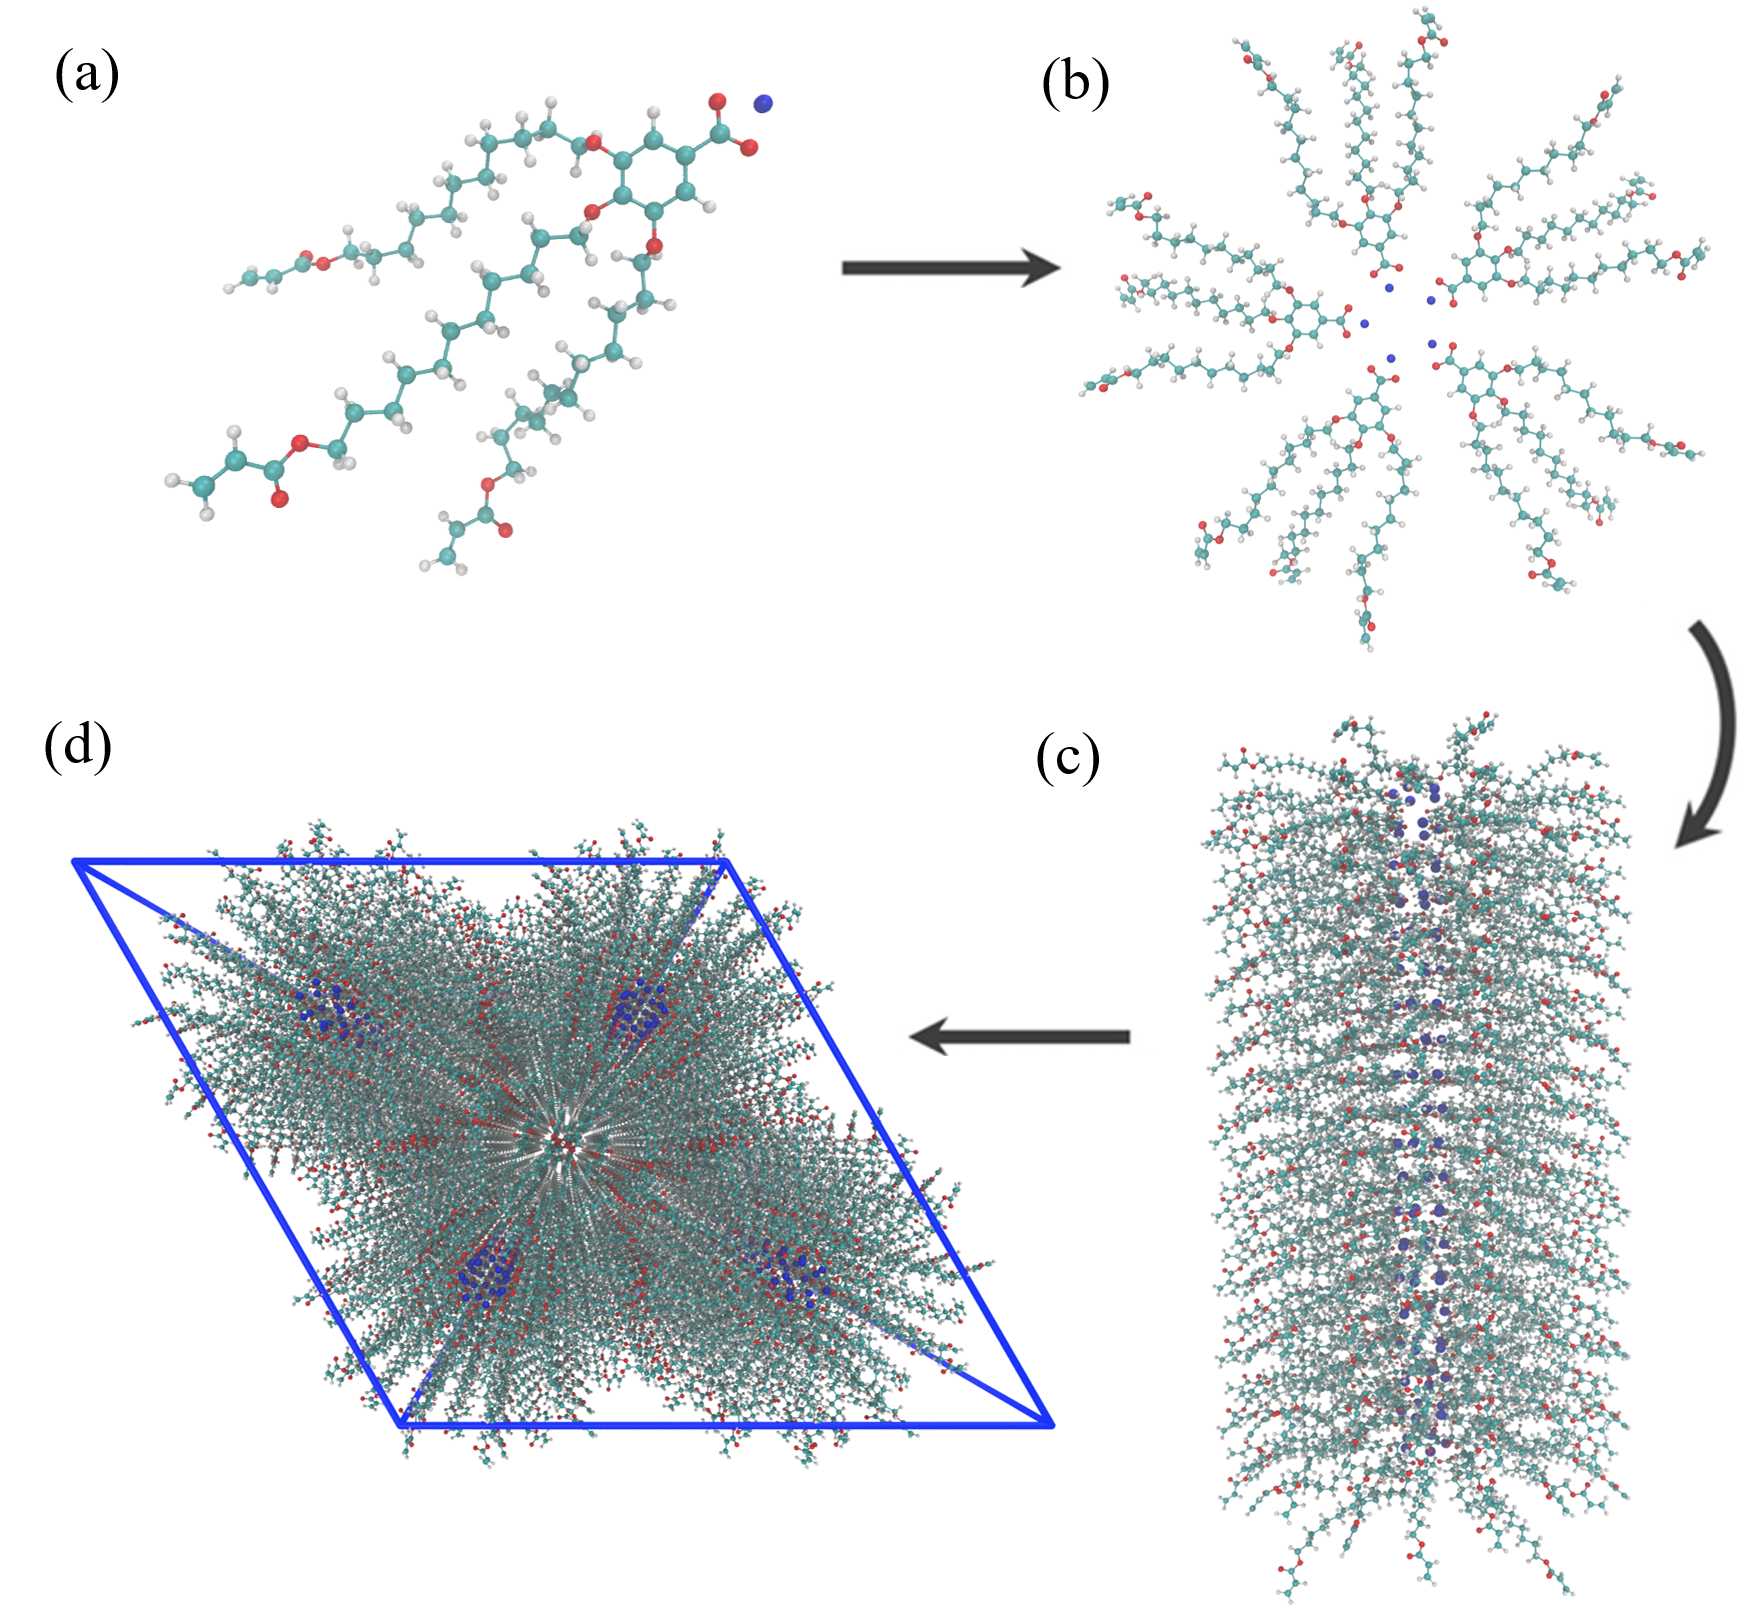
\includegraphics[width=0.75\linewidth]{build.PNG} %BJC: put an xyz axis with the unit cell
	\caption{(a) A single monomer was parameterized and annealed to produce a low energy
		configuration. (b) Monomers are rotated and assembled into layers with 
		hydrophlic centers. (c) Twenty layers are stacked on top of each other to create
		a pore. (d) Pores are duplicated and placed in a monoclinic unit cell}\label{fig:python}
  \end{figure}
  
  A typical simulation volume contains four pores in a monoclinic unit cell,
  the smallest unit cell that maintains hexagonal symmetry when extended 
  periodically.
  \begin{itemize}
    \item Each pore is made of twenty stacked monomer layers with periodic 
    continuity in the z direction, avoiding any edge effects and creating an 
    infinite length pore ideal for studying transport.
    \item A small number of layers is preferred in order to reduce computational
    cost and to allow us to look at longer timescales.
    \item Ultimately, we chose to build a system with 20 monomer layers in each pore
    in order to obtain sufficient resolution when simulating X-ray diffraction patterns.
    This point will be explained in more detail later.
  \end{itemize}
  
  We chose initial guesses for the remaining structural parameters based on 
  experimental data and treated them as variables during model development.
  %BJC: I could potentially break this paragraph into smaller paragraphs centered around
  % the bolded structural parameters
  \begin{itemize}
    \item \textbf{The distance between pores} was based on experimental SAXS data for
    this system \cite{feng_thin_2016}.
    \item The model's pores are spaced 4.5 nm apart initially, $\approx$ 10 \% larger
    than the experimental value of 4.12 nm in order to reduce unintended repulsions 
    resulting from a tightly packed initial configuration.
    \item The layer spacing is based on experimental 2D WAXS data.
    \item The pattern shows reflections corresponding to features spaced 3.7 \angstrom apart.
    \item It has been hypothesized that the features are a result of pi-pi
    interactions between stacked aromatic rings \cite{feng_scalable_2014}. 
    \item Our simulations tend to equilibrate to a wider interlayer spacing of
    $\approx$ 4.1 \angstrom, which inspired separate systems starting with layer 
    spacings greater than 4 \angstrom.
    \item We estimate the \textbf{pore radius} to be 0.6 nm based on past TEM images 
    and size exclusion rejection data\cite{feng_scalable_2014,feng_thin_2016,
    zhou_supported_2005}.
    \item Comparing a geometric measurement of pore size derived from an 
    atomistic model, to a less precise, experimentally derived pore size estimate,
    will give ambiguous results.
    \item What is meant by pore radius will not be clear until we have a clear picture
    of the nanoscopic pore environment.
    \item When constructing pores, we chose the carboxylate carbon from the monomer
    head group as a reference atom, and placed it a distance r from the pore center,
    where r is the pore radius.  %BJC: figure making that clear
    \item We will not make direct comparisons of pore radius between our model 
    and experiment to avoid the ambiguity. 
    \item The \textbf{relative interlayer orientation} was chosen based on clues from 
    diffraction data as well as the various known stacking modes of benzene 
    and substituted benzene rings: sandwiched, parallel-displaced and T-shaped
    ~\cite{sinnokrot_estimates_2002} (\Cref{fig:sandwiched,fig:pd,fig:tshaped}).
    \item The T-shaped configuration was ruled out based on the inconsistency of
    its $\approx$ 5 \angstrom equilibrium stacking distance ~\cite{sinnokrot_estimates_2002}.
    \item The system's preference towards the sandwiched vs. parallel displaced 
    stacking modes will be explored.
    %BJC: I think the following commentary belongs elsewhere, maybe even in the discussion
    \item Visualization of each configuration (\Cref{fig:sandwichedlayers,fig:offsetlayers})
    suggests entropic differences based on the way the tails are able to pack.
    \item In the sandwiched configuration, all tails start out directly on top
    of each other which may prevent closely stacked benzene rings.
    \item In the offset configuration, the tails are placed in between each other 
    which may allow layers to come together in a compact way.
    \item This difference may explain, in part, which stacking mode is more favorable.
  \end{itemize}

  An equilibration scheme with position restraints placed on aromatic rings
  prevents unrealistic jumps during early equilibration steps.
  
  Simulated X-ray diffraction patterns were generated based on atomic
  coordinates for a direct experimental comparison.
  
  \begin{figure}[H]
	\centering
	\begin{subfigure}[b]{0.32\textwidth}
		\centering
		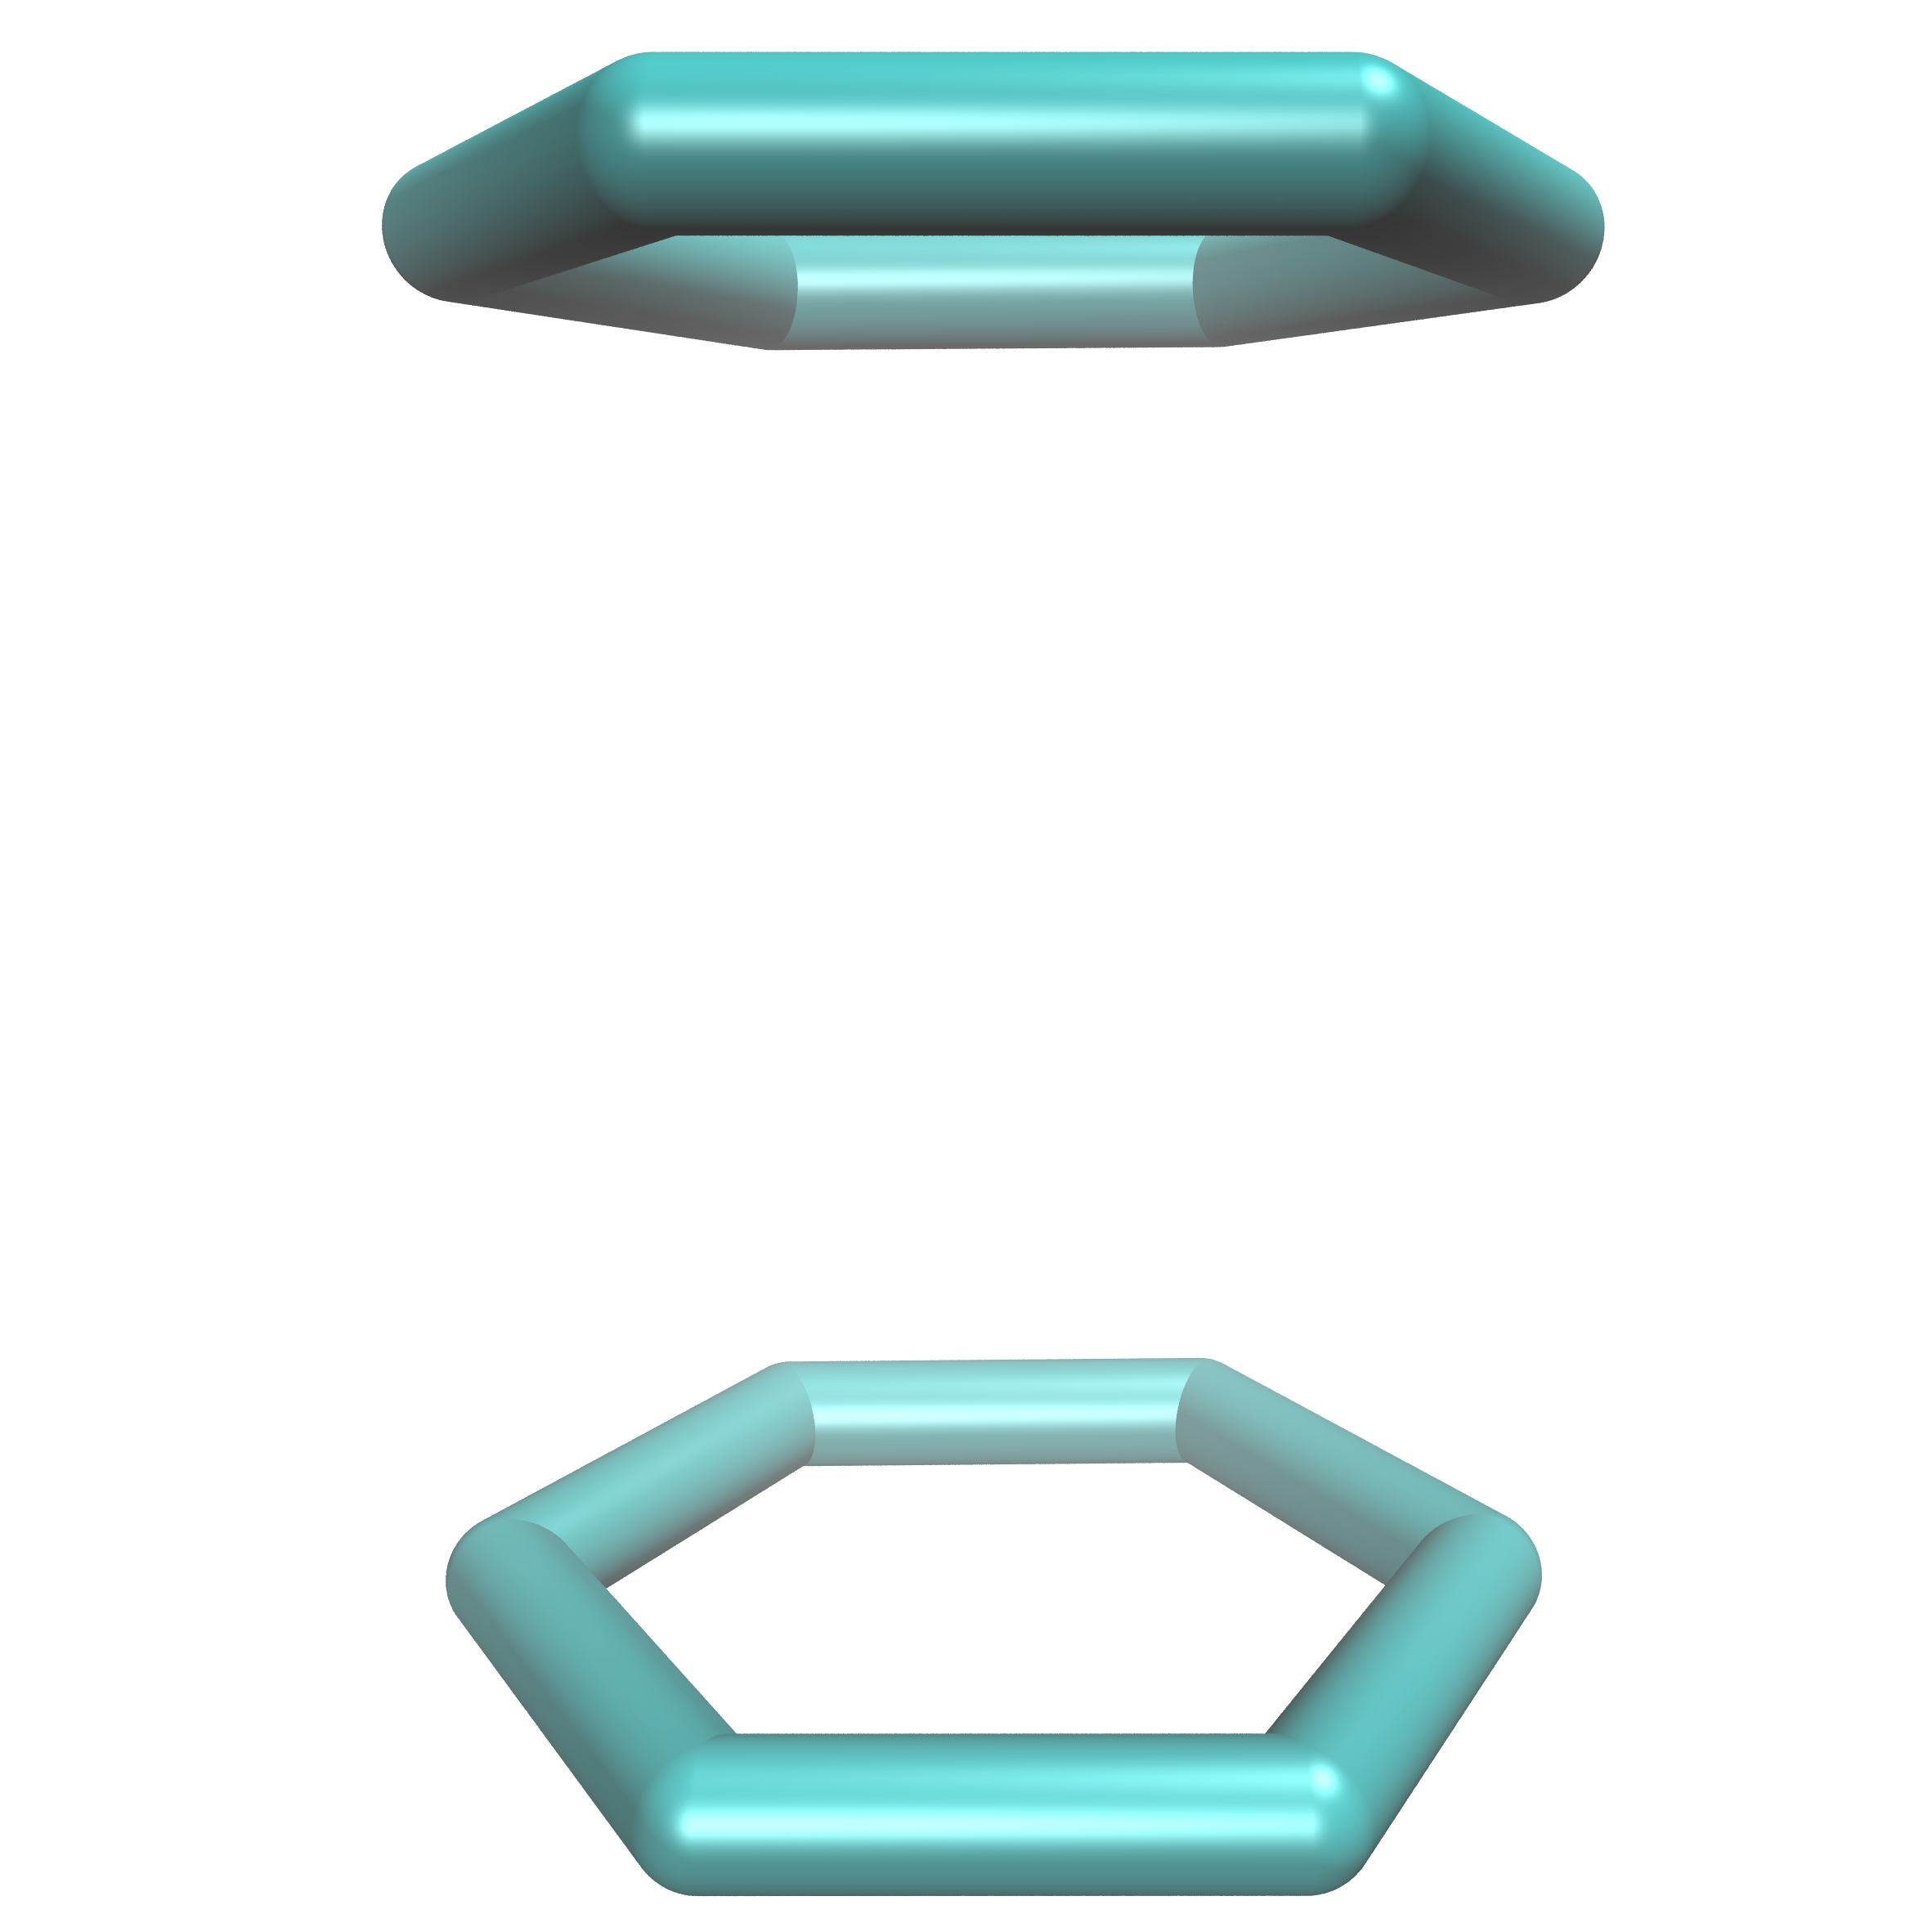
\includegraphics[width=\textwidth]{sandwiched.png}
		\caption{}\label{fig:sandwiched}
	\end{subfigure}
	\begin{subfigure}[b]{0.32\textwidth}
		\centering
		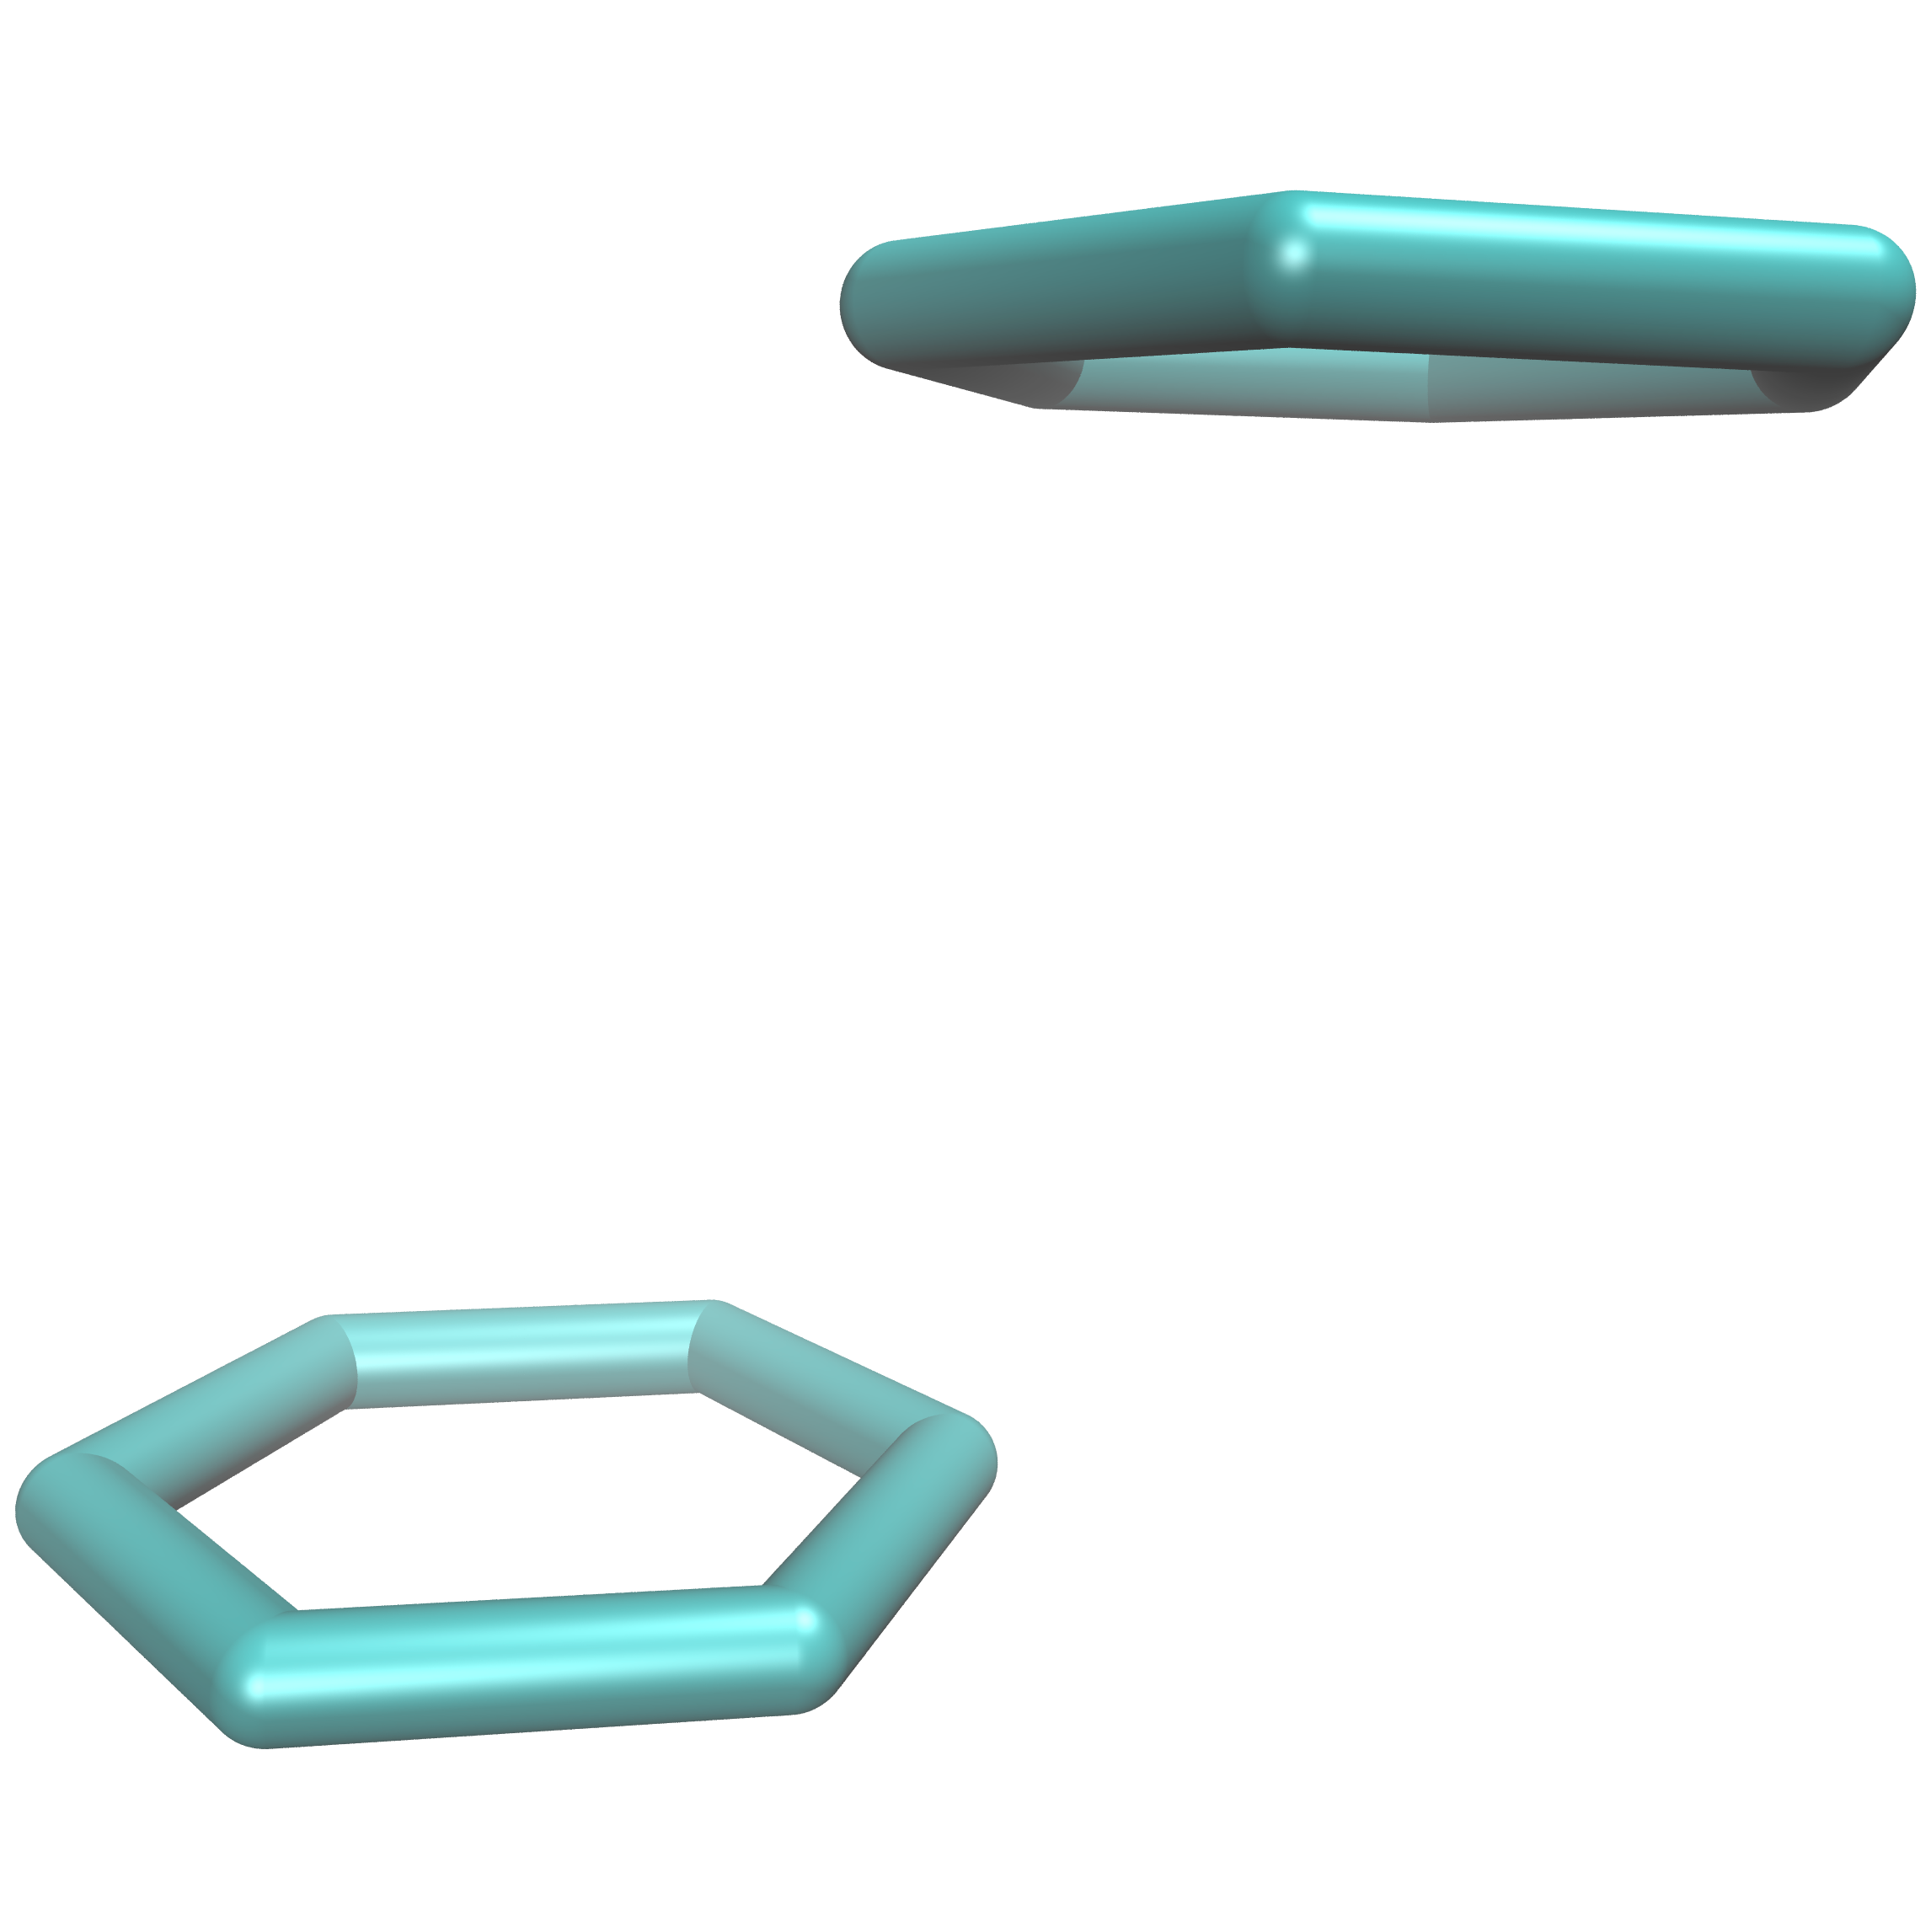
\includegraphics[width=\textwidth]{PD.png}
		\caption{}\label{fig:pd}
	\end{subfigure}
	\begin{subfigure}[b]{0.32\textwidth}
		\centering
		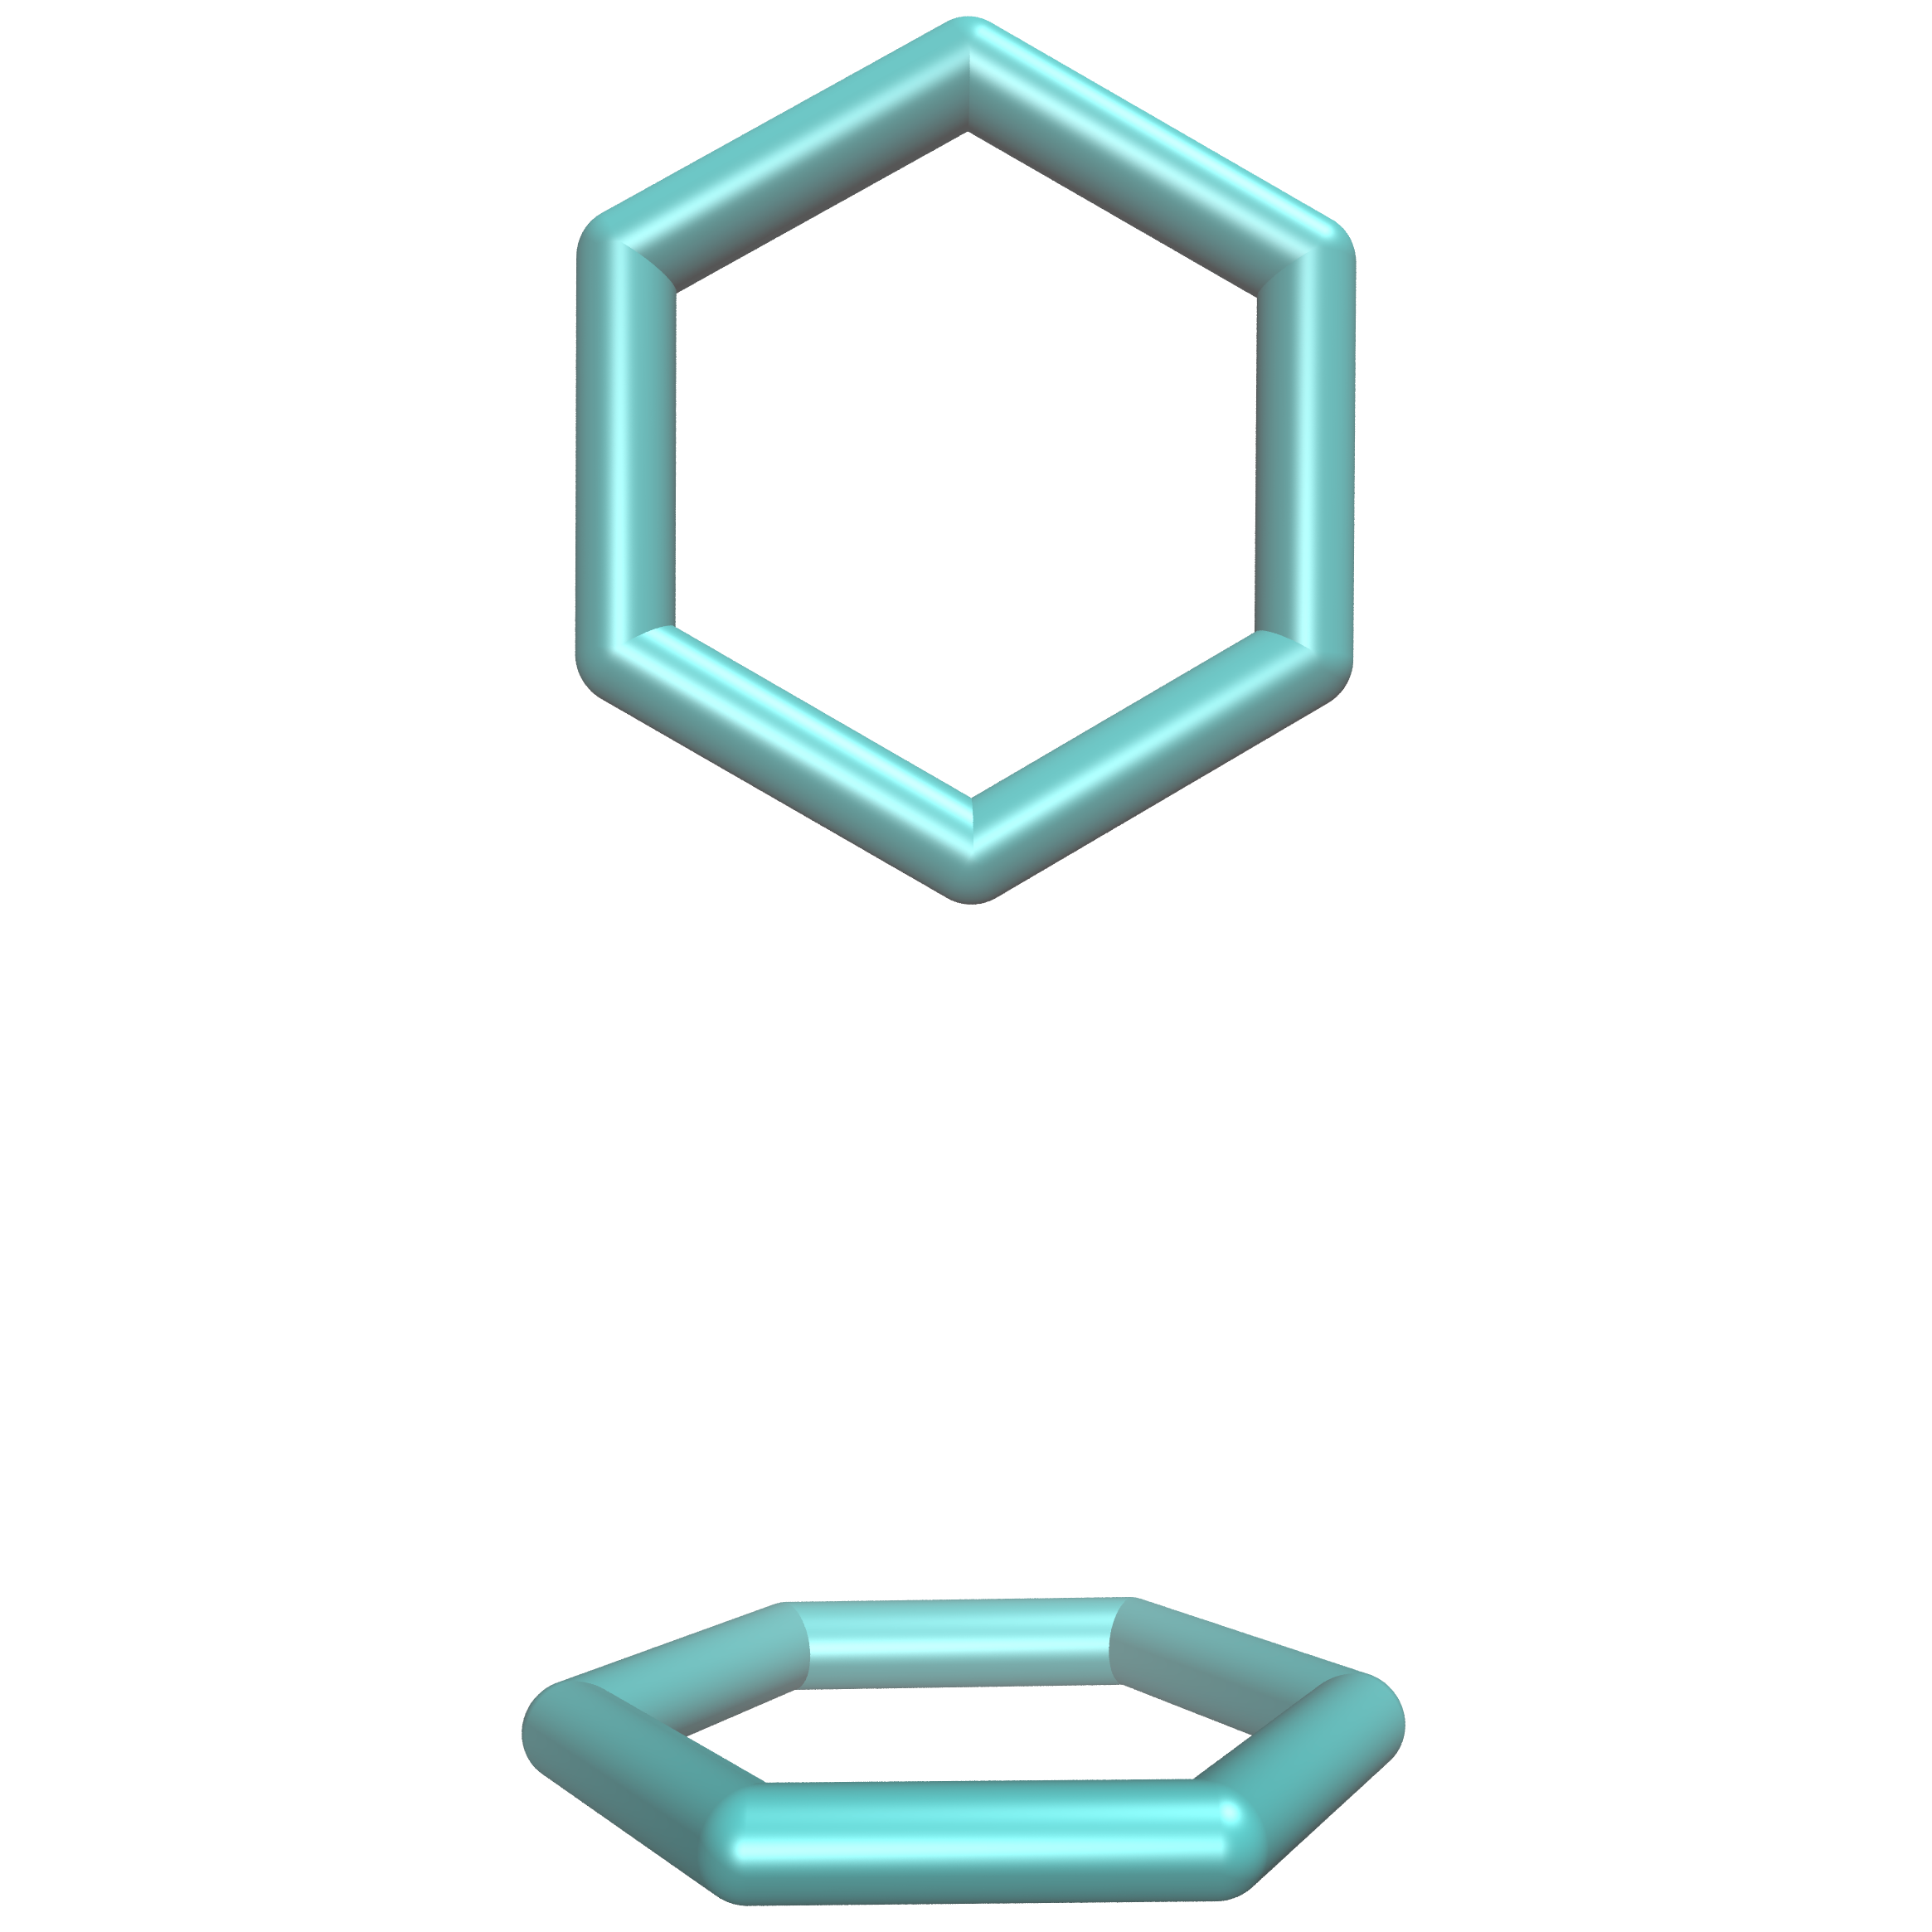
\includegraphics[width=\textwidth]{Tshaped.png}
		\caption{}\label{fig:tshaped}
	\end{subfigure}
	\vskip\baselineskip
	\begin{subfigure}[b]{0.475\textwidth}
		\centering
		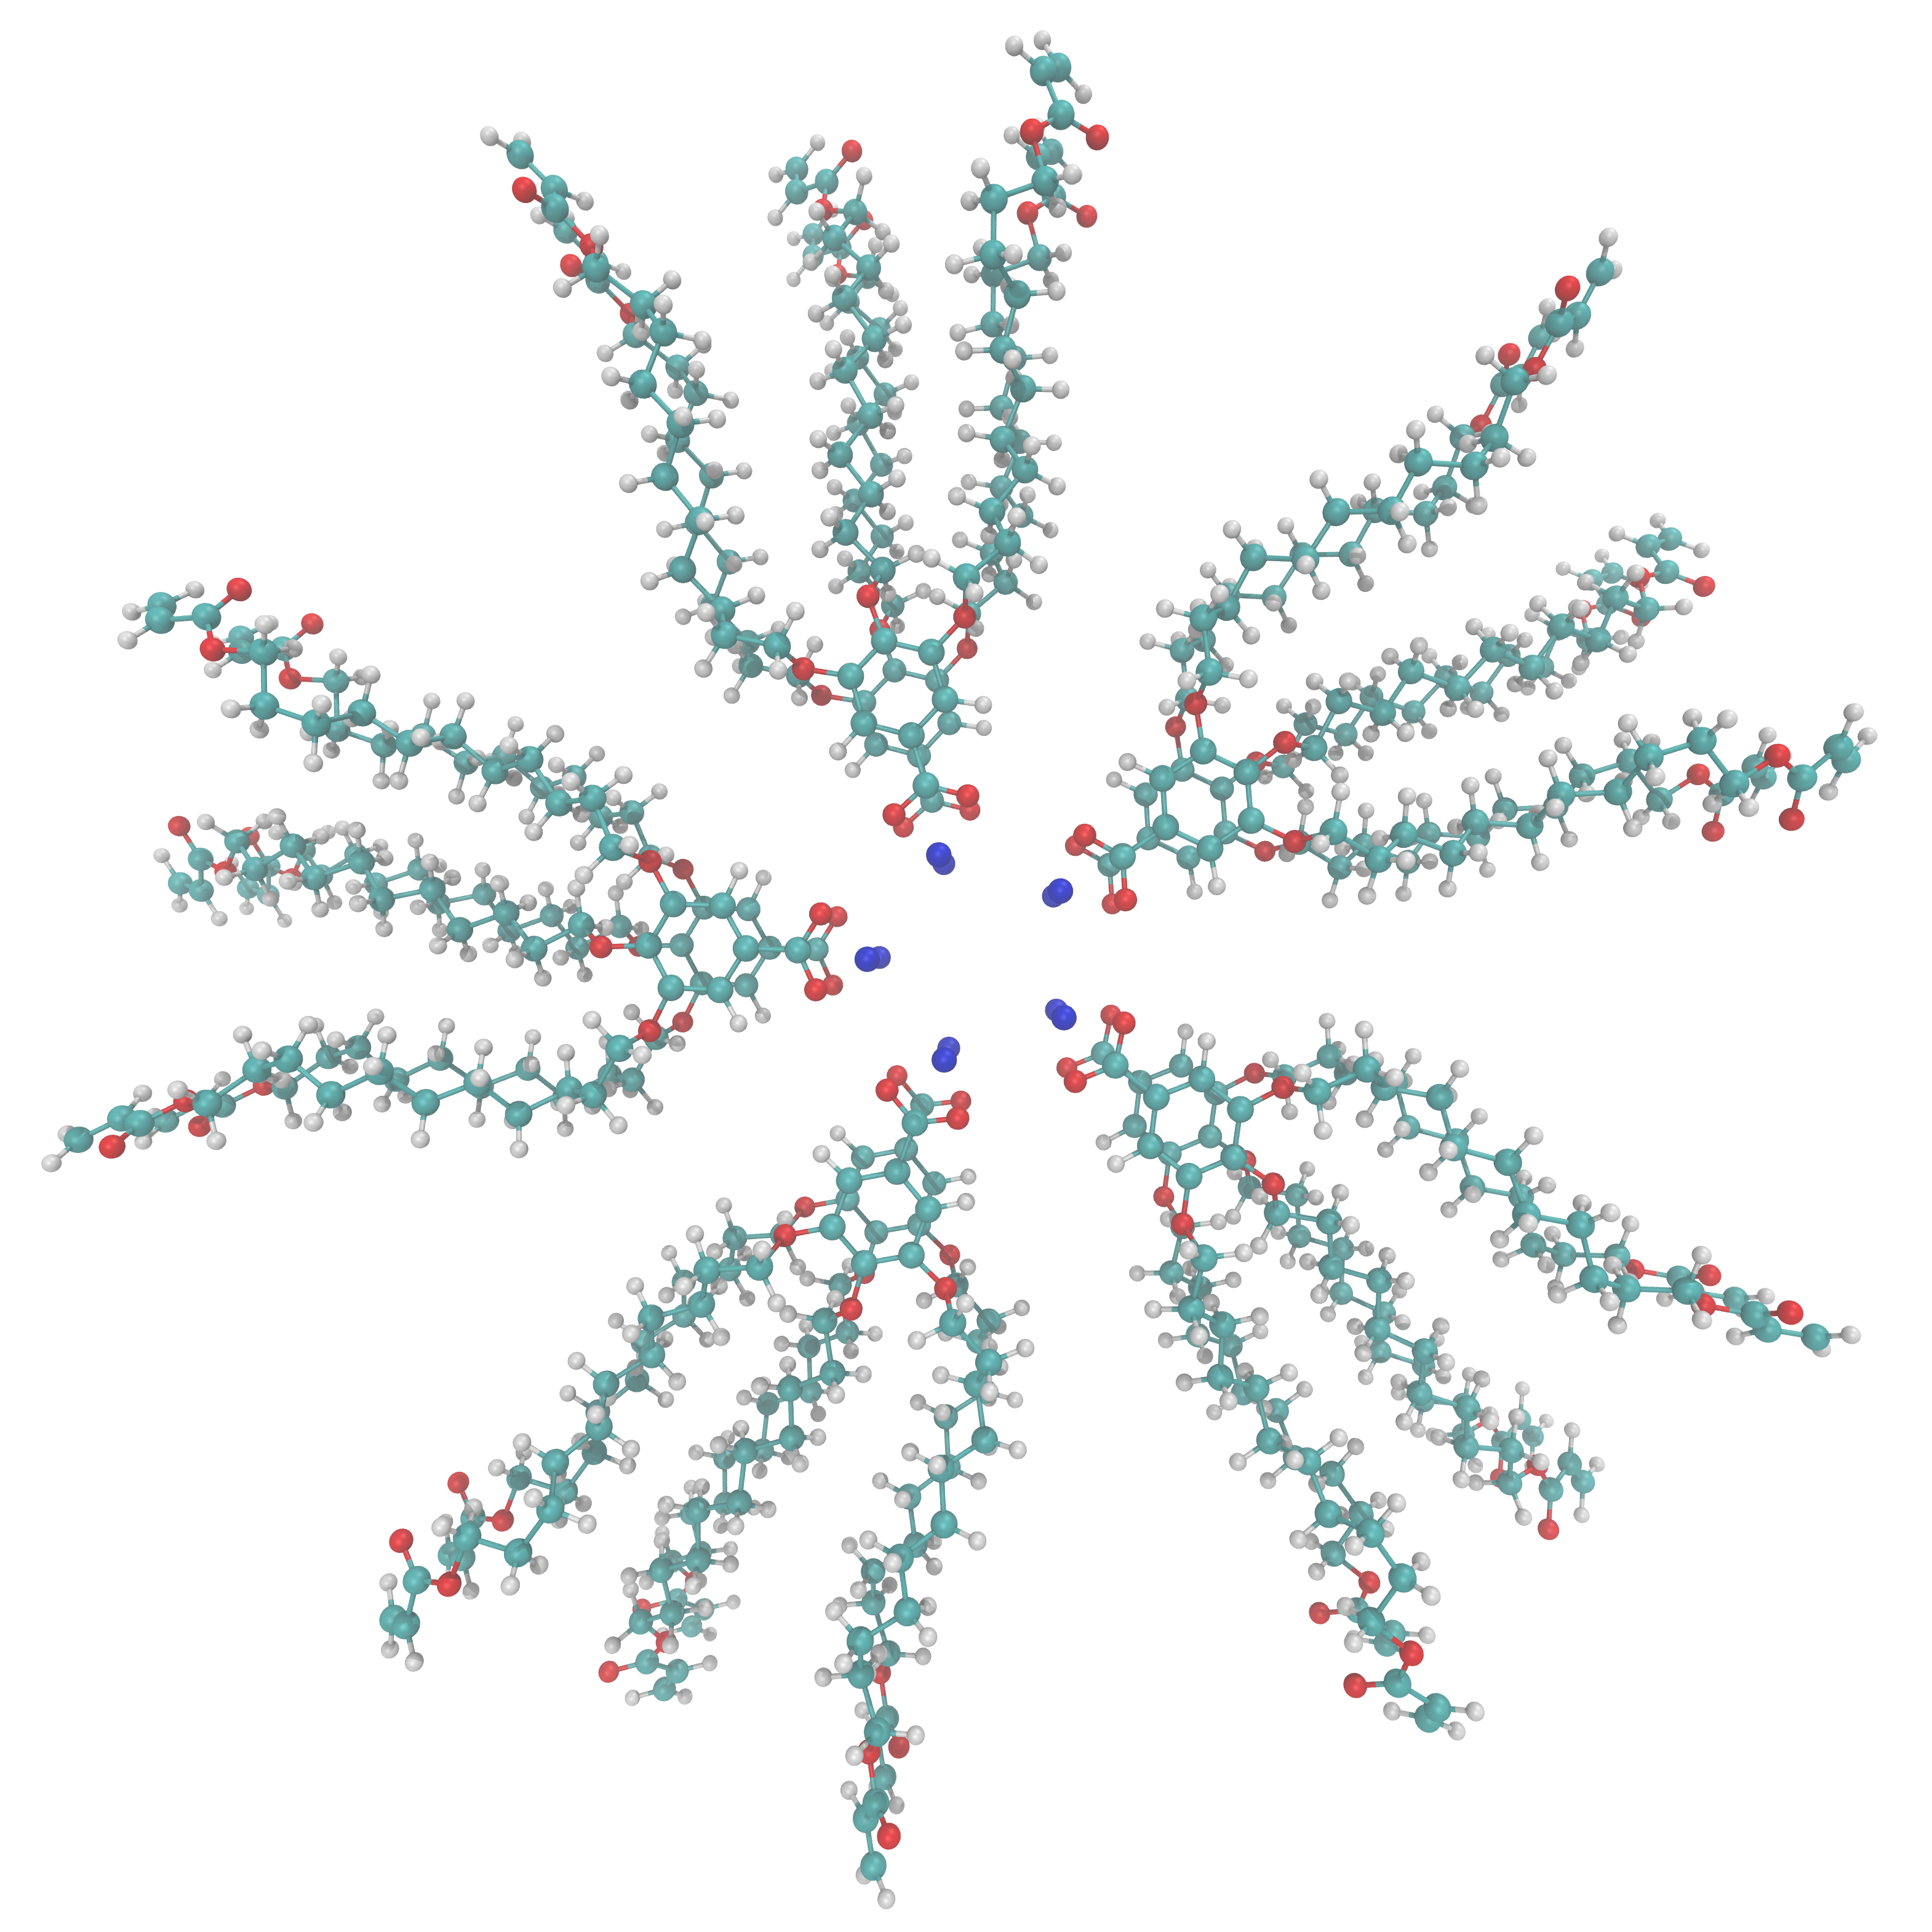
\includegraphics[width=\textwidth]{sandwichedlayers.png}
		\caption{}\label{fig:sandwichedlayers}
	\end{subfigure}
	\begin{subfigure}[b]{0.475\textwidth}
		\centering
		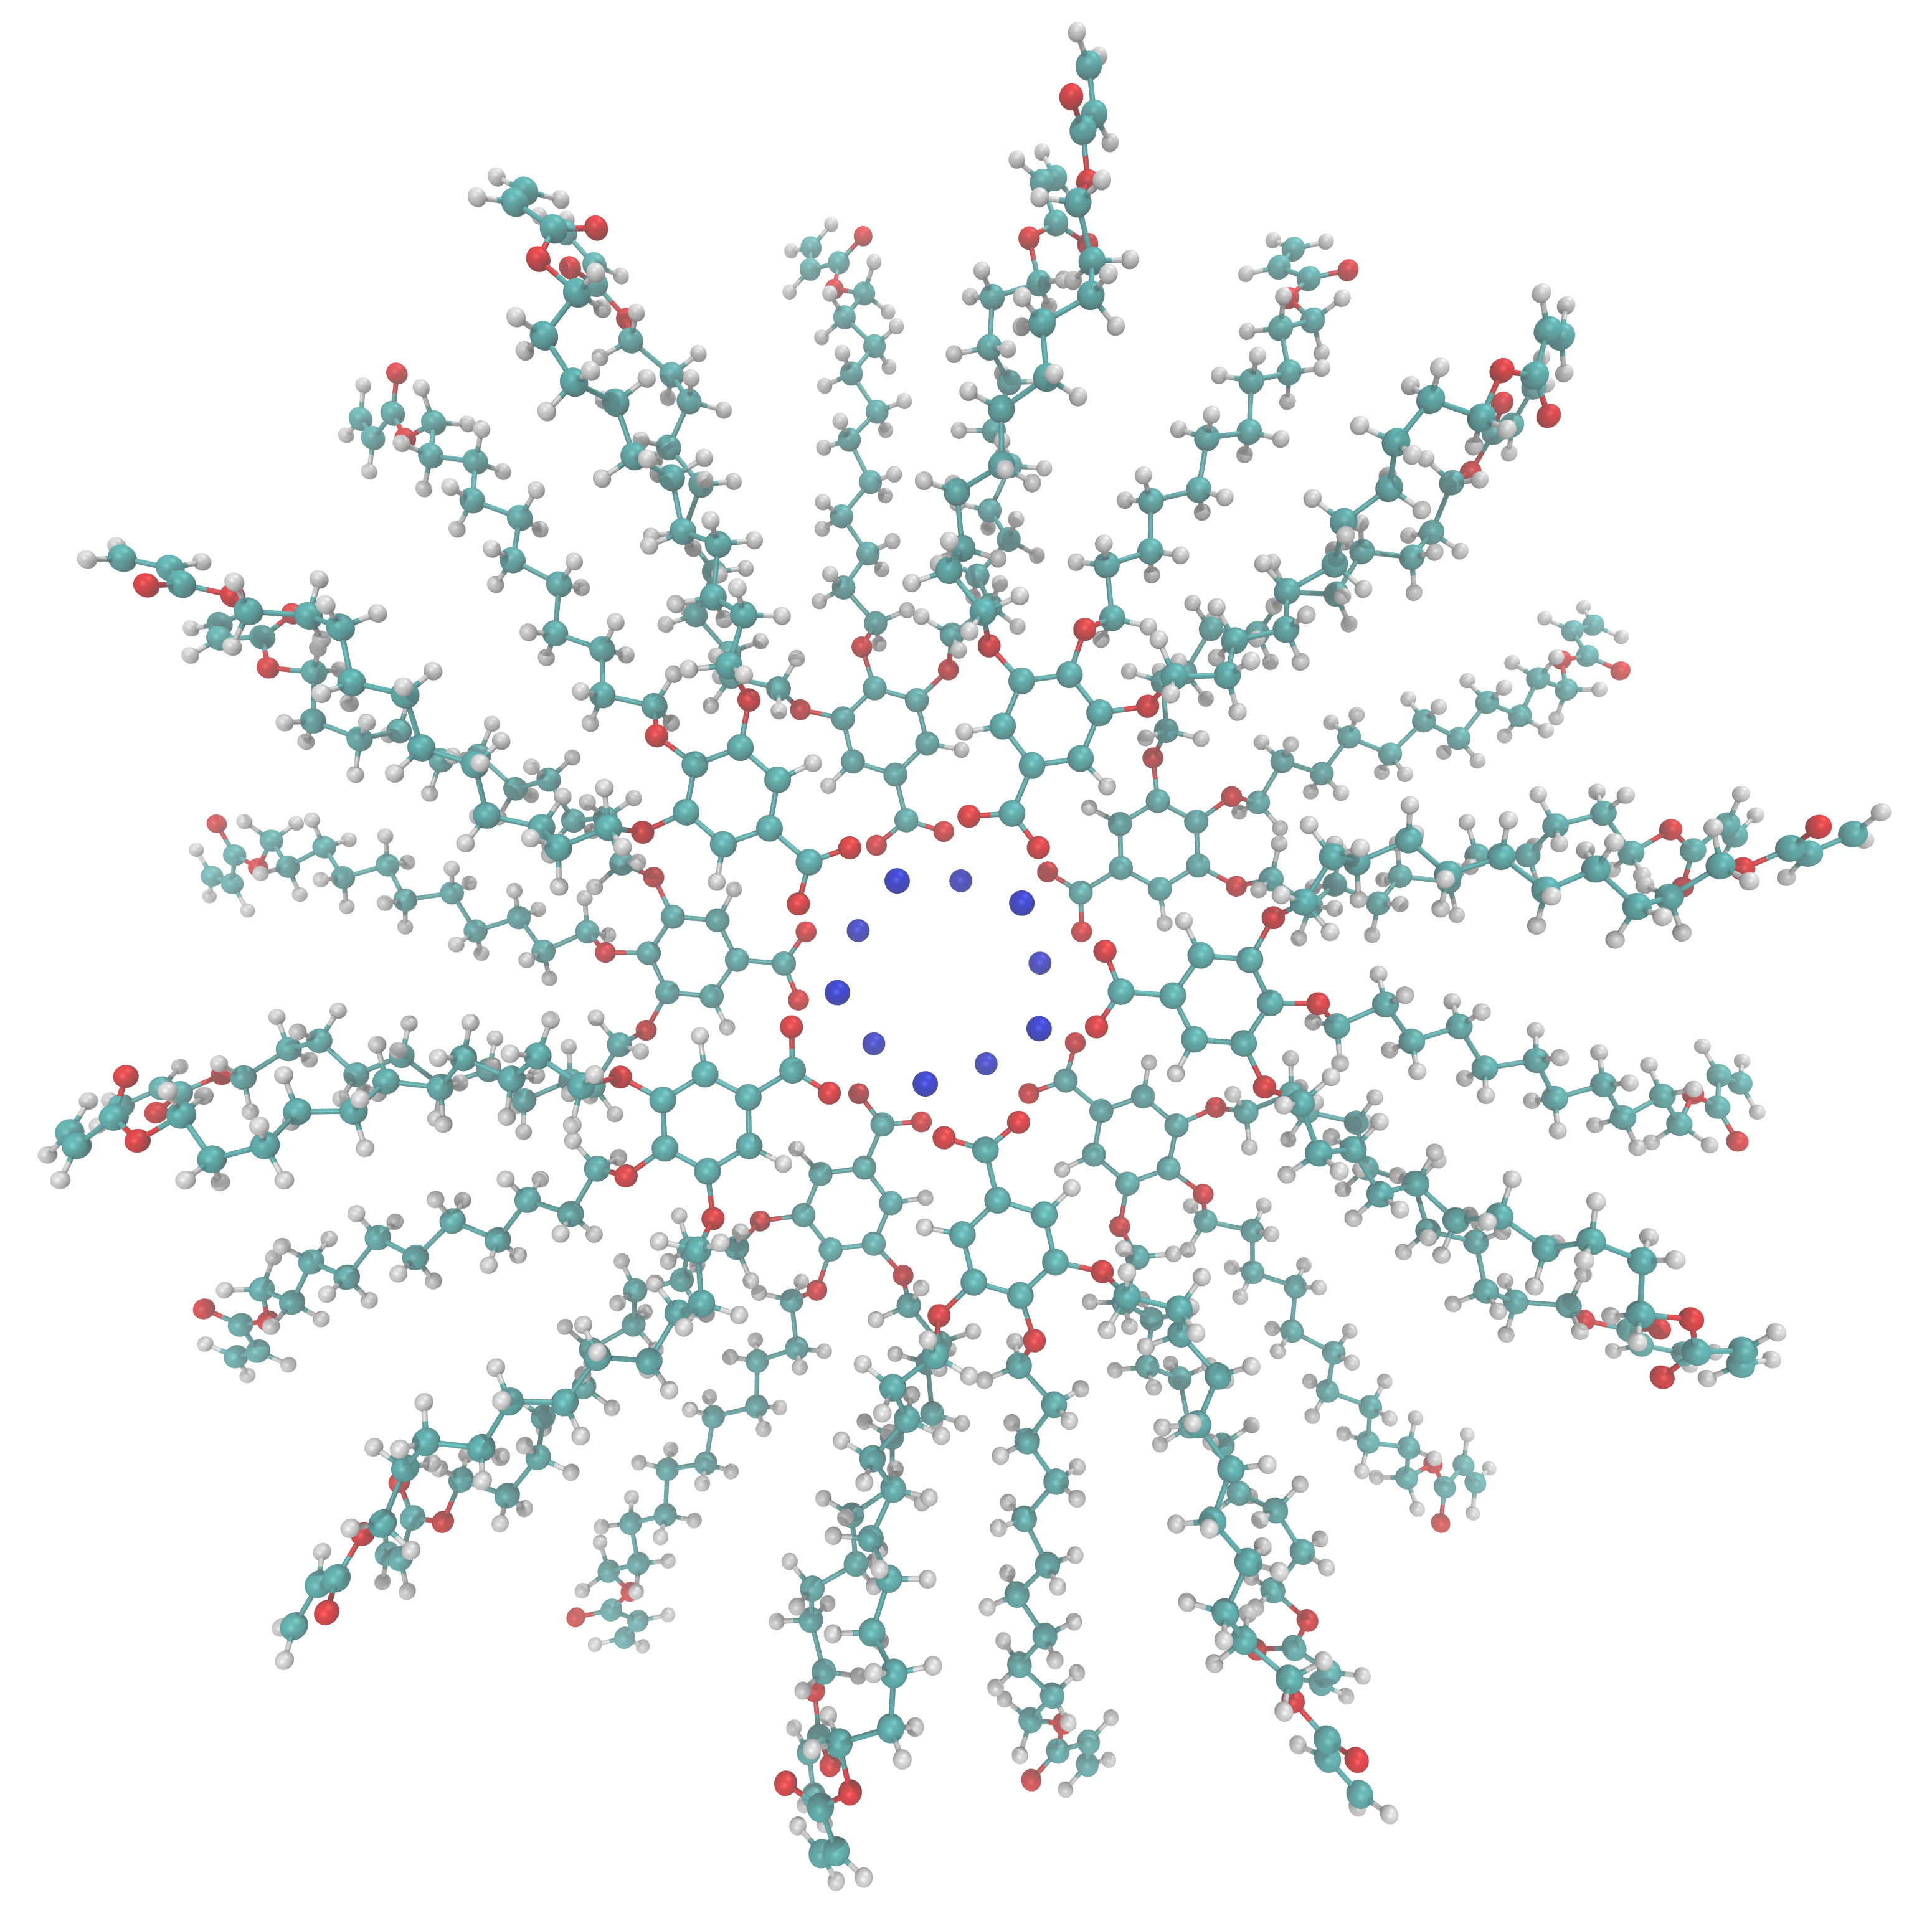
\includegraphics[width=\textwidth]{offsetlayers.png}
		\caption{}\label{fig:offsetlayers}
	\end{subfigure}
	\caption{(a) Sandwiched benzene dimers stack 3.8 \angstrom apart. (b) Parallel-Displaced benzene dimers stack
	3.4 \angstrom vertically and 1.6 \angstrom horizontally apart. (c) T-shaped benzene dimers stack 5.0 \angstrom apart. 
	(d) Two monomer layers stacked in the sandwiched configuration (e) Two monomer layers stacked in the parallel-displaced
	configuration }\label{fig:stacking}
  \end{figure}
  
  Ionic conductivity was calculated using two different methods for
  robustness.
  
  Using an equilibrated structure, a crosslinking procedure was performed
  in order to better parallel synthetic procedures. 
